\documentclass{standalone}

\usepackage{standalone}
\usepackage{tikz}
\usetikzlibrary{er,positioning, calc}

\begin{document}

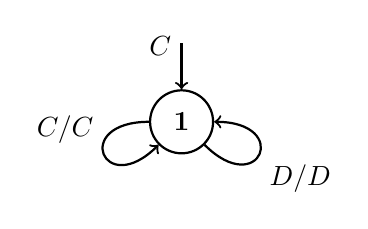
\begin{tikzpicture}
	\tikzstyle{state}=[minimum width=0.8cm, font=\boldmath];

   	\node[circle, draw=black, thick] (0) at (0, 0) [state]    {$1$};
	\coordinate (s) at (0, 1);
    \draw (s) edge[out=-90, in=90, ->, thick] node [above left] {$C$} (0);
    \draw (0) edge[out=180, in=-135, ->, thick, loop, looseness=8] node [above left] {$C/C$} (0);
    \draw (0) edge[out=-45, in=0, ->, thick, loop, looseness=8] node [below right] {$D/D$} (0);
\end{tikzpicture}
\end{document}